% Comparative analysis: four critic/value-based RL papers vs. Flow-Factory PPO.
% Compile: pdflatex ppo_papers_comparison.tex (run twice for refs / hyperref / toc).
% Requires: tikz, algorithm, algpseudocode, booktabs, amsmath, amsthm, hyperref.
\documentclass[11pt]{article}

\usepackage[utf8]{inputenc}
\usepackage[T1]{fontenc}
\usepackage{lmodern}
\usepackage[a4paper,margin=1in]{geometry}
\usepackage{amsmath,amssymb,amsthm,bm}
\usepackage{booktabs}
\usepackage{array}
\usepackage{enumitem}
\usepackage{caption}
\usepackage{xcolor}
\usepackage{algorithm}
\usepackage{algpseudocode}
\usepackage{tikz}
\usetikzlibrary{arrows.meta,positioning,shapes.geometric,calc,fit,backgrounds}
\usepackage[colorlinks=true,linkcolor=blue,citecolor=blue,urlcolor=teal]{hyperref}

\theoremstyle{remark}
\newtheorem{remark}{Remark}

% TikZ shared styles
\tikzset{
  box/.style={draw, rounded corners, align=center, minimum height=0.9cm,
              text width=3.1cm, fill=blue!5, font=\small},
  mech/.style={draw, rounded corners, align=center, minimum height=1.5cm,
              text width=3.5cm, fill=teal!8, font=\small},
  trunk/.style={draw, rounded corners, align=center, minimum height=0.9cm,
              text width=3.4cm, fill=orange!10, font=\small},
  flow/.style={-{Stealth[length=2.5mm]}, thick},
}

\newcommand{\zt}{\bm{z}}
\newcommand{\xt}{\bm{x}}
\newcommand{\E}{\mathbb{E}}
\newcommand{\R}{\mathbb{R}}
\newcommand{\Vphi}{V_\phi}

\title{\textbf{Critic-/Value-based RL for Diffusion \& Flow-Matching Models}\\[2pt]
\large A Comparative Analysis of Four Papers and the Flow-Factory PPO Trainer}
\author{Flow-Factory}
\date{\today}

\begin{document}
\maketitle

\begin{abstract}
This note compares four recent papers on RL fine-tuning of diffusion / flow-matching
generators against Flow-Factory's critic-based PPO trainer (\texttt{trainer\_type:
ppo}). All five methods share a single thesis: replace GRPO's coarse, trajectory-level,
\emph{group-relative} advantage with a learned, timestep-conditioned \emph{state value
function} $\Vphi(\zt_t, t)$ on noisy latents for fine-grained credit assignment. They
diverge along two orthogonal axes: (i)~\textbf{how the value becomes a parameter
update} (the actor mechanism) and (ii)~\textbf{what network realizes the value} (the
critic body). The papers are: \emph{DiffAC}~\cite{zhou2024diffac}
(arXiv:2403.04154), \emph{VARD}~\cite{dai2025vard} (arXiv:2505.15791),
\emph{AC-Flow}~\cite{fan2025acflow} (arXiv:2510.18072), and \emph{Explicit Critic
Guidance}~\cite{liang2026critic} (arXiv:2605.27736). A central, easy-to-miss finding:
\emph{only} Explicit Critic Guidance is also \emph{true} PPO (clipped policy-gradient
surrogate + GAE), like ours; the other three keep a state-value critic but replace the
PPO actor with, respectively, a one-step actor--critic on forward-perturbed states, a
differentiable value back-propagated through the sampler, and an advantage-weighted
flow-matching regression. For each paper we state its unique contribution, its core
equations, and---concretely---how it would be implemented in the Flow-Factory codebase
(what already exists, what is new). The companion note \texttt{docs/ppo/ppo\_analysis}
documents our trainer in depth.
\end{abstract}

\tableofcontents

\section{Scope and the One Shared Idea}
\label{sec:scope}

Flow-Factory fine-tunes flow-matching / diffusion models with online RL against
(typically non-differentiable) reward models. The default algorithm, GRPO, treats a
whole denoising rollout as one ``action'': it computes a single scalar advantage per
sample by \emph{group-relative} reward normalization and broadcasts it to every
denoising step. This is simple and strong but gives no per-step credit and uses a
group-mean (state-blind) baseline.

Every method in this note attacks exactly that limitation with the \emph{same} core
device:

\begin{quote}
\emph{Learn a timestep-conditioned value $\Vphi(\zt_t, t)$ on the noisy latent state
that the policy actually visits, and use it for fine-grained, per-step credit
assignment.}
\end{quote}

Because the reward is terminal-only, the value at any intermediate state is the
\emph{expected final reward given that state}, $\Vphi(\zt_t,t)\approx\E[R\mid\zt_t]$,
and its Monte-Carlo regression target is just the terminal reward $R$. (With
$\gamma=\lambda=1$ even GAE collapses to this Monte-Carlo target at every step.) That
shared skeleton is what makes the five methods comparable; everything interesting is in
\emph{how each one turns $\Vphi$ into a gradient}.

\paragraph{The four papers at a glance.}
Table~\ref{tab:identity} fixes identities. Two are published/peer-track
(DiffAC, ICML 2024) and three are preprints under review. They span UNet, DiT/MMDiT and
SE(3) backbones, and image / molecule / protein tasks, but the recurring testbed is
text-to-image LoRA fine-tuning, which is also our primary use case.

\begin{table}[h]
\centering
\small
\begin{tabular}{p{2.5cm} p{3.3cm} p{2.6cm} p{4.4cm}}
\toprule
\textbf{Short name} & \textbf{Title (abbrev.) / venue} & \textbf{Backbone(s)} & \textbf{Task / reward} \\
\midrule
\textbf{DiffAC}\newline arXiv:2403.04154 &
Stabilizing Policy Gradients for SDEs via Consistency with Perturbation Process;
\emph{ICML 2024} &
TargetDiff (SE(3) diff.); SD1.5 (UNet, LoRA) &
Drug design (Vina); T2I (ImageReward) \\
\addlinespace
\textbf{VARD}\newline arXiv:2505.15791 &
VARD: Efficient and Dense Fine-Tuning with Value-based RL; \emph{preprint} &
SD1.4 / SDXL (UNet); FoldFlow-2 (flow) &
T2I (Aesthetic, PickScore, ImageReward, HPSv2; compressibility); protein \\
\addlinespace
\textbf{AC-Flow}\newline arXiv:2510.18072 &
Fine-tuning Flow Matching Generative Models with Intermediate Feedback; \emph{preprint} &
SD3 (MMDiT, LoRA) &
T2I on DrawBench (CLIP score) \\
\addlinespace
\textbf{Explicit Critic}\newline arXiv:2605.27736 &
Explicit Critic Guidance for Aligning Diffusion Models; \emph{preprint} &
SD1.5 (UNet); SD3.5M (DiT) &
T2I (CLIP, HPSv2.1, PickScore, GenEval, OCR) \\
\addlinespace
\textbf{Flow-Factory PPO}\newline (ours) &
Critic-based PPO (\texttt{trainer\_type: ppo}); see \texttt{ppo\_analysis} &
Model-agnostic (conv / packed / video) &
Any registered reward (terminal weighted sum) \\
\bottomrule
\end{tabular}
\caption{The four papers and our trainer. ``Explicit Critic'' is the paper our team
previously referenced; it is the only one besides ours that is genuine PPO.}
\label{tab:identity}
\end{table}

\paragraph{A naming caveat worth stating up front.}
``Actor--critic'', ``value'', ``advantage'', and ``critic warmup'' appear in all four
papers, but three of them are \emph{not} PPO. Section~\ref{sec:taxonomy} makes the
distinction precise; without it the comparison is misleading.

\section{A Unifying MDP and the Two Axes of Variation}
\label{sec:taxonomy}

\subsection{Denoising as a finite-horizon MDP}
All methods model the ordered sampling steps as an MDP (following DDPO/Flow-GRPO):
state $s_t=(\zt_t, t)$ (a noisy latent plus its timestep; some add the text condition
$y$), action $a_t$ = the next latent $\zt_{t-1}$ (equivalently the predicted denoising
direction), the policy is the per-step transition, and the reward is \emph{terminal
only}, $R=\sum_k w_k\, r_k(\text{decode}(\zt_0))$. The value $\Vphi(\zt_t,t)$ estimates
the expected terminal reward from $\zt_t$, with terminal value $0$. This is exactly the
formulation in our \texttt{ppo\_analysis} note.

\subsection{Axis 1 --- how $\Vphi$ becomes a gradient (the actor mechanism)}
This is the dominant axis. There are four distinct mechanisms across the five methods:

\begin{enumerate}[leftmargin=1.6em]
  \item \textbf{PPO clipped policy gradient} (\emph{Ours}, \emph{Explicit Critic}).
  $\Vphi$ is a \emph{baseline}; GAE turns TD residuals into per-step advantages
  $\hat A_t$; the policy is updated by the clipped importance-ratio surrogate. The
  critic is never differentiated \emph{into} the policy.
  \item \textbf{One-step actor--critic on perturbed states} (\emph{DiffAC}).
  REINFORCE with the \emph{next} state's value as the return
  ($\nabla\!\log\pi\cdot \Vphi(\text{next})$), or DDPG (pathwise $\nabla_\theta\Vphi$).
  States are synthesized by \emph{noising clean samples forward}, not by rollout.
  \item \textbf{Differentiable value back-propagation} (\emph{VARD}). The (reparam.)
  sampler is differentiable, so maximize $\Vphi(\zt_t)$ directly by back-propagating
  its gradient \emph{through} the sampling step into $\theta$ (deterministic policy
  gradient / reward-backprop). No log-probs, no ratio.
  \item \textbf{Advantage-weighted regression} (\emph{AC-Flow}). Sidestep the
  intractable flow-matching likelihood: re-weight the conditional flow-matching (CFM)
  regression loss by $\exp(\tau\hat A_t)$ (an AWR/RWR generalization). No log-probs, no
  ratio.
\end{enumerate}

Figure~\ref{fig:fanout} draws the common trunk and the four branches.

\begin{figure}[h]
\centering
\resizebox{\textwidth}{!}{%
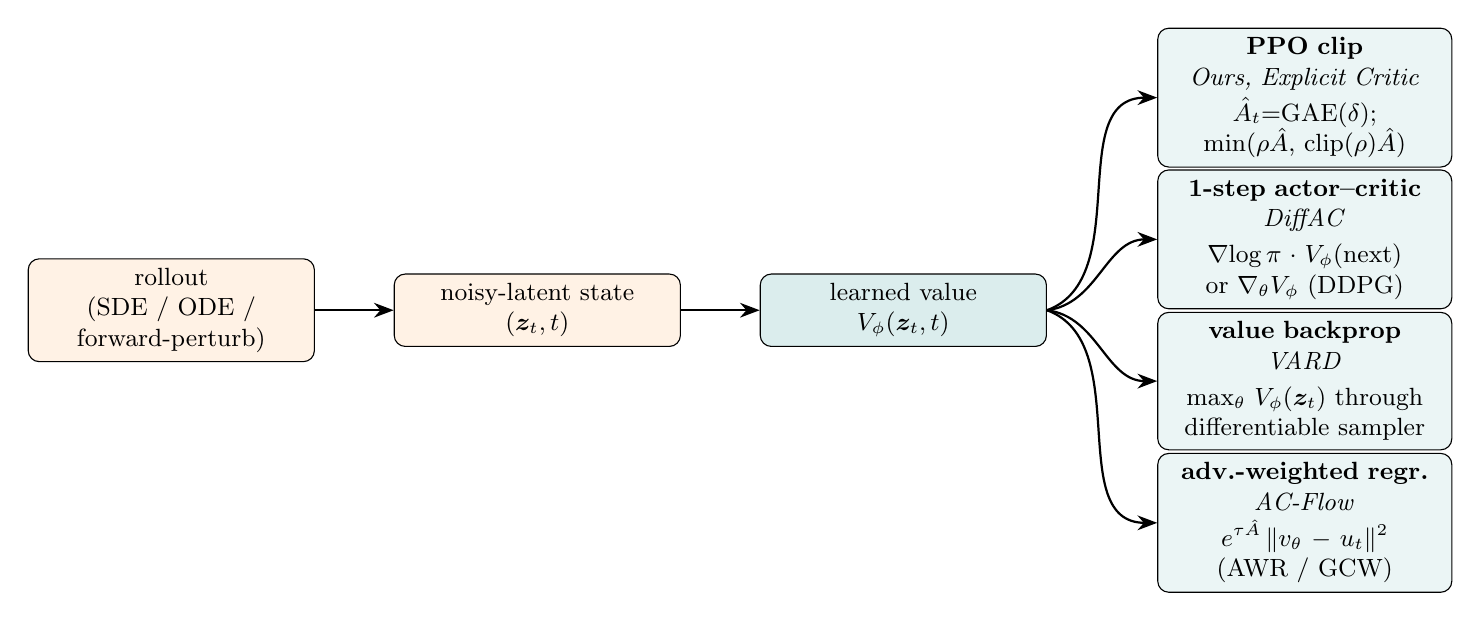
\begin{tikzpicture}[node distance=0.5cm and 1.0cm]
  \node[trunk] (roll) {rollout\\ (SDE / ODE / forward-perturb)};
  \node[trunk, right=of roll] (state) {noisy-latent state\\ $(\zt_t, t)$};
  \node[trunk, right=of state, fill=teal!14] (val) {learned value\\ $\Vphi(\zt_t, t)$};
  \draw[flow] (roll) -- (state);
  \draw[flow] (state) -- (val);

  \node[mech, right=1.4cm of val, yshift=2.7cm] (ppo)
    {\textbf{PPO clip}\\ \emph{Ours, Explicit Critic}\\[2pt]
     $\hat A_t{=}\mathrm{GAE}(\delta)$;\\
     $\min(\rho\hat A,\,\mathrm{clip}(\rho)\hat A)$};
  \node[mech, right=1.4cm of val, yshift=0.9cm] (ac)
    {\textbf{1-step actor--critic}\\ \emph{DiffAC}\\[2pt]
     $\nabla\!\log\pi\cdot\Vphi(\mathrm{next})$\\ or $\nabla_\theta\Vphi$ (DDPG)};
  \node[mech, right=1.4cm of val, yshift=-0.9cm] (vard)
    {\textbf{value backprop}\\ \emph{VARD}\\[2pt]
     $\max_\theta\,\Vphi(\zt_t)$ through\\ differentiable sampler};
  \node[mech, right=1.4cm of val, yshift=-2.7cm] (awr)
    {\textbf{adv.-weighted regr.}\\ \emph{AC-Flow}\\[2pt]
     $e^{\tau\hat A}\,\lVert v_\theta-u_t\rVert^2$\\ (AWR / GCW)};

  \draw[flow] (val.east) to[out=20,in=180] (ppo.west);
  \draw[flow] (val.east) to[out=7,in=180] (ac.west);
  \draw[flow] (val.east) to[out=-7,in=180] (vard.west);
  \draw[flow] (val.east) to[out=-20,in=180] (awr.west);
\end{tikzpicture}%
}
\caption{One shared value $\Vphi(\zt_t,t)$, four ways to turn it into a parameter
update. Only the top branch (ours and Explicit Critic) is PPO.}
\label{fig:fanout}
\end{figure}

\subsection{Axis 2 --- what network is the critic (the critic body)}
\begin{itemize}[leftmargin=1.6em]
  \item \textbf{Independent lightweight net}: \emph{Ours} (token-fold + residual MLP +
  learned-query attention pooling + sinusoidal time), \emph{AC-Flow} (CNN+MLP),
  \emph{DiffAC} (backbone-shaped for molecules; T2I head unspecified).
  \item \textbf{The diffusion backbone itself}: \emph{Explicit Critic} (value heads on
  the shared backbone; the policy \emph{is} the critic body).
  \item \textbf{The reward model}: \emph{VARD} (LoRA-adapt the reward model into the
  value net; a plain MLP head was reported insufficient for preference rewards).
\end{itemize}

The two axes are independent: ours and Explicit Critic share Axis~1 (PPO) but sit at
opposite ends of Axis~2 (lightweight independent net vs.\ backbone-as-critic). This
2$\times$ split is the backbone of the per-paper analysis below.

\section{Per-paper Contribution and Flow-Factory Implementation}
\label{sec:papers}

Each subsection gives (a)~the \emph{unique} contribution, (b)~the core method/equations,
(c)~the relation to our trainer, and (d)~a concrete implementation mapping to the
codebase (\texttt{trainers/ppo/\{trainer,gae,critic\}.py},
\texttt{hparams/training\_args/ppo.py}).

\subsection{DiffAC --- consistency with the perturbation process (arXiv:2403.04154)}
\label{sec:diffac}

\paragraph{Unique contribution.}
\begin{enumerate}[leftmargin=1.6em]
  \item \textbf{Forward-perturbation (off-policy) gradient estimation.} Instead of
  estimating the policy gradient on sparse \emph{backward} rollouts, DiffAC
  \emph{noises the generated clean samples $\xt_0$ forward} to synthesize an unlimited,
  space-covering set of intermediate states $\xt_t\sim p_{t0}(\cdot\mid\xt_0)$. Under a
  \emph{consistency} condition (Lemma 4.2) these perturbed states follow the true
  rollout marginal, so the gradient is well-defined and low-variance even in high
  dimensions.
  \item \textbf{Consistency enforced by a score-matching--refit reference + KL}
  (Eqs.\ 12--13), with a formal error bound (Thm 4.5: gradient error $\le$ sum of
  per-step $\sqrt{\mathrm{KL}}$ between the consistent and the policy SDE).
  \item \textbf{A value critic trained by direct Monte-Carlo regression to the terminal
  reward} (Eq.\ 8), and a single framework instantiable with either a REINFORCE or a
  \emph{DDPG/pathwise} actor.
\end{enumerate}

\paragraph{Core method.}
Critic target (with $\xt_t$ a \emph{forward-perturbed} state):
\begin{equation}
\phi^\star=\arg\min_\phi \E_{t,\;\xt_0\sim q_0,\;\xt_t\sim p_{t0}(\cdot\mid\xt_0)}
  \big(\Vphi(\xt_t,t)-R(\xt_0)\big)^2 ,
  \qquad \Vphi^\star(\xt_t,t)=\E_{\xt_0\sim q_{0t}(\cdot\mid\xt_t)}[R(\xt_0)].
\end{equation}
Actor (one SDE step $\bar\xt_{t-\mathrm{d}t}$ from a perturbed $\xt_t$):
\begin{align}
\text{SDE-REINFORCE (Eq.\,10):}\quad
  &\textstyle\mathrm{PG}(\theta)=\frac1n\sum_j
   \nabla_\theta\log P_\theta(\bar\xt_{t-\mathrm{d}t}^j\mid\xt_t^j)\,
   \Vphi(\bar\xt_{t-\mathrm{d}t}^j,\,t{-}\mathrm{d}t),\\
\text{SDE-DDPG (Eq.\,11):}\quad
  &\textstyle\mathrm{PG}(\theta)=\frac1n\sum_j \nabla_\theta \Vphi(\bar\xt_t^j,\,t{-}\mathrm{d}t),\\
\text{Update (Eq.\,13):}\quad
  &\theta\leftarrow\theta+\eta_1\,\mathrm{PG}(\theta)
   -\eta_1\eta_2\,\nabla_\theta D_{\mathrm{KL}}(\varepsilon_\theta,\varepsilon_{\theta'},\mathcal D),
\end{align}
where $\varepsilon_{\theta'}$ is a reference \emph{re-fit by score matching} on the
latest data each iteration. There is \textbf{no GAE and no PPO clip}; the only trust
region is the consistency KL.

\paragraph{Relation to ours.}
Shared: SDE-as-MDP, terminal-only reward, a $V(\xt_t,t)$ critic, a KL-to-reference, and
critic pretraining. Different: DiffAC trains both critic and actor on
\emph{forward-perturbed} states (we use on-policy rollout latents), uses a
\emph{re-fit} reference (ours is a fixed/EMA reference), offers a \emph{pathwise} actor
(we are strictly likelihood-ratio), and uses a \emph{one-step} value signal (we use
multi-step GAE). With $\gamma=\lambda=1$ our GAE return equals DiffAC's MC critic
target --- but evaluated on rollout vs.\ perturbed states.

\paragraph{Implementation in Flow-Factory.}
DiffAC's \emph{actor} is neither PPO-clip nor GAE, so a faithful port is a
\textbf{sibling trainer} (e.g.\ \texttt{trainers/diffac/}) reusing our infrastructure,
not an edit to the PPO loss. Two scoped options:
\begin{itemize}[leftmargin=1.6em]
  \item \textbf{Option A (faithful).} \emph{New}: a forward-perturbation state sampler
  ($\xt_t=\texttt{scheduler.add\_noise}(\xt_0,\,\text{noise},\,t)$, needs a forward-marginal
  helper on the adapter); a one-step actor loss (REINFORCE
  $-\E[\log P_\theta(\bar\xt\mid\xt_t)\,\Vphi(\bar\xt).\mathrm{detach}()]$ or DDPG
  $-\E[\Vphi(\bar\xt)]$); a per-iteration score-matching re-fit of the reference. The
  critic loss becomes plain MSE to $R(\xt_0)$ (drop \texttt{value\_clip\_range}, GAE,
  whitening). \emph{Reused}: \texttt{generate\_samples} rollout + per-step log-prob,
  \texttt{\_compute\_terminal\_rewards}, dual optimizers, critic-warmup scaffolding,
  checkpointing, \texttt{\_compute\_kl} plumbing (extended to refit the reference).
  \item \textbf{Option B (cheap, additive --- recommended follow-up).} Keep our PPO+GAE
  actor, add a \texttt{critic\_target: \{gae, perturb\_terminal\}} switch. In
  \texttt{perturb\_terminal} mode, regress the critic on forward-perturbed states to
  $R(\xt_0)$ (DiffAC Eq.\ 9); GAE then bootstraps off a better-calibrated, lower-variance
  value. A self-contained change to \texttt{\_compute\_old\_values} /
  \texttt{\_critic\_value\_loss} / \texttt{\_fit\_critic\_only} plus a perturbation
  sampler and one hparam. The forward-noising itself is \emph{already implemented} in
  \texttt{trainers/awm.py} (\texttt{noised\_latents = (1 - sigma) * clean\_latents + sigma
  * noise}), so the change is small. This follow-up is written up in full---plan,
  hparams, and caveats (Monte-Carlo target only, timestep-scale alignment, consistency
  gap)---in \texttt{docs/ppo/ppo\_analysis} \S\,``Follow-up: DiffAC-style perturbed-state
  critic training''.
\end{itemize}
New hparams (Option A): \texttt{actor\_estimator: reinforce|ddpg},
\texttt{consistency\_kl\_coef} ($\eta_2$), \texttt{reference\_refit\_steps},
\texttt{perturb\_t\_distribution}, off-policy buffer toggle.

\subsection{VARD --- back-propagating a learned dense value (arXiv:2505.15791)}
\label{sec:vard}

\paragraph{Unique contribution.}
\begin{enumerate}[leftmargin=1.6em]
  \item \textbf{A learned value as a differentiable surrogate reward that you
  back-propagate.} Reward-backprop methods (DRaFT/ReFL) need a \emph{differentiable
  reward}; policy-gradient methods (DDPO/DPOK) tolerate non-differentiable rewards but
  are high-variance. VARD trains a value/PRM that is differentiable \emph{even when the
  reward is not}, then back-props \emph{the value} through the sampler --- getting stable
  analytic gradients for non-differentiable rewards. This dissolves the
  ``non-differentiable reward $\leftrightarrow$ stable training'' dilemma.
  \item \textbf{Dense per-step supervision via a Monte-Carlo value} (Eqs.\ 7--8): the
  value predicts the expected final reward from any intermediate state, turning a
  sparse terminal reward into a dense signal \emph{without} TD/GAE.
  \item \textbf{MSE-as-KL (Lemma 1):} per-step output-MSE between fine-tuned and
  pretrained models is gradient-equivalent to the per-step Gaussian KL, a cheap anchor
  that resists reward hacking.
  \item \textbf{Practical recipe:} LoRA-adapt the \emph{reward model} into the value
  net; a DPOK-style plain MLP head was insufficient for preference rewards.
\end{enumerate}

\paragraph{Core method.}
\begin{align}
\text{Value (Eq.\,7):}\quad
  &\Vphi(\xt_{T-t},c)=\E\big[\textstyle\sum_{t'\ge t}R\mid\xt_{T-t'}\big]
   =\E[\text{final reward}\mid\xt_{T-t}], \\
\text{Value pretraining (Eq.\,8):}\quad
  &J(\phi)=\E\big[(r(\xt_0,c)-\Vphi(\xt_{T-t},c))^2\big]\quad\text{(Monte-Carlo)}, \\
\text{Policy (Eq.\,9):}\quad
  &J(\theta)=-\E\big[\,\Vphi(\xt_{T-t},c)+\eta\lVert \xt_{T-t}-\xt^0_{T-t}\rVert^2\big],\\
\text{MSE$\leftrightarrow$KL (Eq.\,10):}\quad
  &\nabla_\theta\,\E\lVert\xt_{T-t}-\xt^0_{T-t}\rVert^2
   =2\sigma^2\,\nabla_\theta D_{\mathrm{KL}}(p_\theta\Vert p_{\theta_0}).
\end{align}
The gradient flows through the differentiable value and the reparameterized sampler
into $\theta$. \textbf{No importance ratio, no PPO clip, no GAE}; requires a
differentiable sampler. Images fine-tune only the final 10 of 50 steps.

\paragraph{Relation to ours.}
Strongly shared ingredients: MDP, terminal reward, a separate value net, the
\emph{Monte-Carlo} value target (our \texttt{compute\_gae} with $\gamma=\lambda=1$ gives
exactly returns $\equiv R$ at every step), value pretraining + online refresh (our
\texttt{critic\_warmup\_steps} + periodic re-warmup), and the \emph{$x$-space KL anchor}
(our \texttt{kl\_type="x-based"}, $\eta\leftrightarrow$\texttt{kl\_beta}). The crux
difference: VARD's \emph{policy update is value backprop through the sampler} (the value
is the objective), whereas ours uses the value as a \emph{detached baseline} in a
score-function PPO gradient.

\paragraph{Implementation in Flow-Factory.}
Add a \texttt{policy\_objective: \{ppo-clip, value-backprop\}} mode (or a
\texttt{VARDTrainer}); it reuses $\sim$70\% of our scaffolding but swaps the policy loss.
\emph{No trainer in the repo currently does differentiable-rollout reward backprop}, so
this is genuinely new infrastructure.
\begin{itemize}[leftmargin=1.6em]
  \item \textbf{Reused as-is:} value warmup/refresh ($=$ VARD Stage~1 + online value
  fine-tune); the MC value target ($\gamma{=}\lambda{=}1$); the $x$-based KL/MSE anchor
  (\texttt{\_compute\_kl}, $\eta\leftrightarrow$\texttt{kl\_beta}); the reference model
  (\texttt{use\_ref\_parameters}); last-$k$-step training (\texttt{train\_timesteps} /
  \texttt{compute\_trajectory\_indices}). The scheduler's
  \texttt{next\_latents\_mean} is already differentiable w.r.t.\ policy params.
  \item \textbf{Main change (\texttt{optimize}):} replace the PPO-clip block. Forward the
  policy step \emph{with grad} (do not detach \texttt{next\_latents}); compute
  $\Vphi(\text{next})$ \emph{with grad enabled}; loss
  $=-\Vphi(\text{next}).\mathrm{mean}()+\texttt{kl\_beta}\cdot\mathrm{MSE}$. Remove the
  ratio/clip/advantage path. A per-step single-step backprop keeps memory bounded.
  \item \textbf{Critic body (optional, recommended):} a mode to use a LoRA-adapted
  reward model as the value net (our \texttt{ValueCritic} is the cheaper fallback they
  found weaker).
  \item \textbf{Hparams:} \texttt{policy\_objective}; reuse \texttt{kl\_beta} as $\eta$
  (note the paper sweeps $\eta\in[0.1,100]$); in this mode, validate that ratio/GAE
  knobs are inert (fail-fast on misconfig).
\end{itemize}
\textbf{Caveat:} backprop through the backbone per step is more memory-hungry than our
log-prob replay (paper mitigates via last-10-steps + LoRA + grad-accum); it needs a
differentiable sampler (true for our flow scheduler's \texttt{next\_latents\_mean}).

\subsection{AC-Flow --- advantage-weighted flow-matching regression (arXiv:2510.18072)}
\label{sec:acflow}

\paragraph{Unique contribution.}
\begin{enumerate}[leftmargin=1.6em]
  \item \textbf{Generalized Critic Weighting (GCW).} The flow-matching likelihood is
  intractable ($\nabla\!\cdot v_\theta$ is \#P-hard), so AC-Flow replaces the
  policy-gradient update with an $\exp(\tau\cdot\text{signal})$-weighted \emph{CFM
  regression} that unifies RWR ($\Psi{=}r$), AWR/GRAE ($\Psi{=}(r{-}\mu)/\sigma$), and
  critic-advantage ($\Psi{=}r{-}V$) --- and instantiates it with a per-state
  \emph{critic advantage} for intermediate feedback.
  \item \textbf{A dual-stability recipe} that makes online flow actor--critic converge
  where naive value regression diverges (actor loss $10^{12}\!\to\!10^2$):
  \emph{min--max reward shaping} (Eq.\ 6), \emph{advantage clipping} ($\pm\delta{=}5$),
  and a \emph{GRAE-weighted critic warm-up} (actor keeps training with group-relative
  weights while the critic matures, $k{=}500$).
  \item \textbf{Wasserstein-2 (velocity-$L^2$) regularization} (Thm 3.3) in place of
  the intractable KL, with a cheap CNN+MLP critic ($\sim$2\,GB / $\sim$2\,h overhead).
\end{enumerate}

\paragraph{Core method.}
Sampling is \emph{deterministic ODE}; ``intermediate states'' are CFM interpolations
$\xt_t=t\,\xt_1+(1-t)\,\xt_0$ with target $u_t=\xt_1-\xt_0$.
\begin{align}
\text{Reward shaping (Eq.\,6):}\;\;
  &\mathrm{RS}(r_i)=\frac{r_i-\min(r)}{\max(r)-\min(r)+\epsilon}, \\
\text{Critic (Eq.\,10):}\;\;
  &L_{\mathrm{critic}}=\E\big[(\Vphi(\xt_t,t,c)-\mathrm{RS}(r))^2\big],
   \qquad A=\mathrm{RS}(r)-\Vphi(\xt_t,t,c), \\
\text{Actor (Eqs.\,11--12):}\;\;
  &L_{\mathrm{actor}}=\E\big[e^{\tau\,\mathrm{clip}(A,\pm\delta)}\lVert v_\theta-u_t\rVert^2\big]
   +\alpha\!\int_0^1\!\E\lVert v_\theta-v_{\theta_{\mathrm{ref}}}\rVert^2\,\mathrm ds.
\end{align}
\textbf{No importance ratio, no PPO clip, no GAE, no per-step log-probs}; the advantage
is one-sample Monte-Carlo $A=r-V$ (a ``GAE-inspired'' family is described but not used).

\paragraph{Relation to ours.}
Shared: a separate lightweight time-conditioned scalar critic; advantage clipping at
$\pm 5$ (our \texttt{adv\_clip\_range}); a velocity-$L^2$ reference penalty (our
\texttt{kl\_type="v-based"} $=$ their $W_2$ surrogate); a critic warmup; separate
backward passes. Different: AC-Flow's \emph{actor is advantage-weighted CFM regression}
(not a ratio loss), the advantage is \emph{MC} not GAE, it uses \emph{min--max reward
shaping} (we whiten advantages instead), an \emph{exp-weight temperature} $\tau$, a
\emph{GRAE-weighted} warmup (we freeze the policy during bootstrap), and ODE sampling
(no per-step log-prob storage).

\paragraph{Implementation in Flow-Factory.}
A new actor-loss mode (\texttt{policy\_objective: gcw}) on \texttt{PPOTrainer}, or a
sibling trainer (conceptually the reward-weighted/RWR flow trainer $+$ a critic weight).
\begin{itemize}[leftmargin=1.6em]
  \item \textbf{Reward (\texttt{prepare\_feedback}):} add min--max reward shaping
  $\mathrm{RS}(r)$ over the global batch; new hparam \texttt{reward\_norm:
  \{none, minmax, whiten\}}.
  \item \textbf{Advantage (\texttt{gae.py}):} add an MC mode
  ($A=\mathrm{RS}(r)-V$, returns $=\mathrm{RS}(r)$); a
  \texttt{compute\_mc\_advantage} helper selected by \texttt{advantage\_mode:
  \{gae, mc\}}. Keep the existing $\pm 5$ advantage clip.
  \item \textbf{Actor (\texttt{optimize}):} the main new code --- replace the ratio block
  with $w=\exp(\tau\,\mathrm{clip}(A,\pm\delta))$,
  $L_{\mathrm{actor}}=\mathrm{mean}(w\cdot\lVert v_\theta-u_t\rVert^2)$. The adapter
  must expose the velocity $v_\theta$ and CFM target $u_t=\xt_1-\xt_0$ (a
  \texttt{return\_kwargs=["velocity","cfm\_target"]}-style output). New hparam
  \texttt{gcw\_temperature} ($\tau{=}1$).
  \item \textbf{Regularizer:} already covered --- \texttt{kl\_type="v-based"},
  \texttt{kl\_beta}$=\alpha=1.0$.
  \item \textbf{Warmup:} optional \texttt{warmup\_uses\_grae} (first $k{=}500$ steps use
  $w=\exp(\tau\,(\mathrm{RS}(r)-\mu_B)/\sigma_B)$) instead of our frozen-policy bootstrap.
\end{itemize}
\textbf{Simplification:} this mode needs \emph{no} SDE rollout and \emph{no} per-step
log-prob storage --- ODE sampling $+$ random-$t$ interpolation suffice, so it can be
cheaper than our PPO path.

\subsection{Explicit Critic Guidance --- the diffusion backbone as its own value
function (arXiv:2605.27736)}
\label{sec:explicit}

\paragraph{Unique contribution.}
\begin{enumerate}[leftmargin=1.6em]
  \item \textbf{Backbone-as-value-function on noisy latents.} Convert the pretrained
  diffusion model into a timestep-conditioned scalar critic $\Vphi(\zt_t,t,y)$ with
  lightweight heads (UNet: patchify $+$ learnable summary token $+$ attention head; DiT:
  critic-attention branches at layers 7/15/23 with AdaLN time modulation), initialized
  from the actor. This is \emph{state-aligned} (it scores the actual noisy latents,
  unlike pixel-space critics that decode an OOD $\hat\xt_0$ proxy), and reported
  2.6--4.3$\times$ cheaper than CLIP/BLIP/HPS critics at higher reward.
  \item \textbf{Two simple stabilizers:} AdaLN timestep conditioning on the value head
  (essential in ablation) and a \emph{short} value-pretraining warmup (more is worse:
  GenEval $0.54\!\to\!0.64$ at 15 it, then declines).
  \item \textbf{Inference-time steering for free:} the PPO-trained critic's latent
  gradient $g_t=\nabla_{\zt_t}\Vphi(\zt_t,t,y)$ is injected into the sampler (DDIM:
  $\hat\varepsilon=\varepsilon-\eta\sqrt{1-\bar\alpha_t}\,g_t$; flow:
  $\hat v=v+\eta\,g_t$), requiring no extra training.
  \item \textbf{Multi-reward via per-reward value heads} (shared backbone, one head per
  reward); separate heads beat a shared head and mitigate reward hacking.
\end{enumerate}

\paragraph{Core method.}
\emph{This is true PPO.} Standard GAE (Eqs.\ 7--8) with $\gamma{=}\lambda{=}1$ (pure
Monte-Carlo over short terminal-reward trajectories), global advantage normalization
(Eq.\ 6, clip $[-10,10]$), value-target clip $[-5,5]$, the clipped policy surrogate with
a tiny ratio clip ($10^{-5}$ for SD1.5, $10^{-4}$ for SD3.5M, same high-dim Gaussian
reasoning as ours), and value pretraining (Eq.\ 2). KL-to-base is discussed and
\emph{discarded} (it only shifts the optimization timescale, not the hacking);
mitigation is multi-reward $+$ early stopping.

\paragraph{Relation to ours.}
This is the closest match: same MDP, terminal reward, terminal value $0$, GAE with the
same TD recursion, global advantage whitening, clipped policy ratio, value pretraining,
advantage clamping, CFG-free, one sample per prompt. The decisive difference is
\textbf{Axis 2}: their critic \emph{is} the diffusion backbone (shared weights, text
conditioning, AdaLN), whereas ours is an independent lightweight net conditioned on
$(\zt_t,t)$ only. They also add inference-time steering and per-reward heads, which we
do not have. Our \texttt{ppo\_analysis} already names this ``diffusion-model-as-value''
direction as the backbone+value-head critic we evaluated and deferred --- this paper is
direct evidence the deferred direction pays off.

\paragraph{Status: implemented (core).}
Flow-Factory now ships this paper's critic as \texttt{critic\_type=backbone\_branches}
(\texttt{DiTBranchCritic}): per-layer critic-attention branches at \texttt{critic\_tap\_layers}
(default layers $7/15/23$) with AdaLN timestep modulation, reading the actor backbone's
intermediate features with no critic LoRA, trained with the unchanged PPO+GAE+value-pretraining
machinery and the paper preset ($\gamma=\lambda=1$, value-target clip $[-5,5]$, advantage clip
$[-10,10]$, CFG-free, $40$ SDE steps; \texttt{examples/ppo/lora/sd3\_5/explicit\_critic.yaml}).
Single-reward, SD3.5M, DDP. The inference-time $\nabla_{\zt}V$ steering and per-reward value
heads remain deferred.

\paragraph{Implementation in Flow-Factory.}
Because we are already PPO+GAE, this is the one paper we adopt by \emph{extending}, not
replacing, the trainer. The GAE code, dual-optimizer scaffolding, value warmup,
advantage whitening, value clipping and checkpointing \emph{all carry over unchanged};
only the critic body and a few features are new.
\begin{itemize}[leftmargin=1.6em]
  \item \textbf{Backbone-critic mode (\texttt{critic\_type: \{independent, backbone\}}).}
  In \texttt{\_initialization}, for \texttt{backbone} build value heads on the adapter
  backbone (DiT: critic-attention branches at layers 7/15/23 with AdaLN; UNet:
  summary-token attention head), \emph{initialized from the actor}; the
  \texttt{critic\_optimizer} trains the head params (and optionally the backbone-as-critic
  copy). Swap \texttt{self.critic(latents, t, channel\_dim)} in
  \texttt{\_compute\_old\_values} and \texttt{optimize} for the backbone+head forward
  (passing prompt embeds). Memory caveat: $\sim$2$\times$ a forward per value query;
  reuse cached features where possible.
  \item \textbf{Inference-time steering.} A sampler hook computing
  $g_t=\nabla_{\zt_t}\Vphi$ and injecting it (velocity: $v\mathrel{+}=\eta g_t$; noise:
  $\varepsilon\mathrel{-}=\eta\sqrt{1-\bar\alpha_t}g_t$); new \texttt{steer\_eta}. Pure
  inference feature, but depends on the backbone critic.
  \item \textbf{Multi-reward heads.} Stop pre-summing in
  \texttt{\_compute\_terminal\_rewards}; keep a per-reward vector $R^{(m)}$; $M$ value
  heads; run \texttt{compute\_gae} per reward; store
  \texttt{step\_advantages}/\texttt{step\_returns} per reward; sum the per-head value
  losses. Builds on our source-aware \texttt{advantage\_processor.reward\_weights}.
  \item \textbf{Smaller tweaks:} AdaLN time conditioning on the (independent) critic
  head; optional text conditioning (the paper found time conditioning matters most);
  a paper-faithful preset \texttt{gae\_lambda=1.0} and value-target clip $[-5,5]$.
\end{itemize}

\section{Side-by-side Comparison}
\label{sec:tables}

Tables~\ref{tab:algo} and~\ref{tab:systems} place all five methods on the two axes and
the secondary design choices. Read together with Figure~\ref{fig:fanout}.

\begin{table}[h]
\centering
\footnotesize
\setlength{\tabcolsep}{4pt}
\begin{tabular}{p{2.3cm} p{2.3cm} p{2.3cm} p{2.3cm} p{2.3cm}}
\toprule
\textbf{Aspect} & \textbf{Ours (PPO)} & \textbf{DiffAC} & \textbf{VARD} & \textbf{AC-Flow} \\
\midrule
Actor mechanism & PPO clipped PG & 1-step AC (REINFORCE / DDPG) & value backprop (DPG) & adv.-weighted CFM regr.\ (GCW) \\
Importance ratio / clip & yes ($\pm10^{-4}$) & no & no & no \\
Credit assignment & GAE($\gamma,\lambda$) & one-step value & dense value (MC) & MC advantage $r{-}V$ \\
Critic target & GAE returns, clipped & MC $\to R$ (perturbed states) & MC $\to R$ & MC $\to \mathrm{RS}(r)$ \\
Reward normalization & advantage whitening & none & none & min--max shaping \\
Regularization to base & optional KL ($v$/$x$) & consistency KL (refit ref) & MSE-as-KL (Lemma 1) & $W_2$ velocity-$L^2$ \\
Is it PPO? & \textbf{yes} & no & no & no \\
\bottomrule
\end{tabular}
\caption{Algorithmic structure (Axis 1). Explicit Critic shares our column (true PPO +
GAE) and is therefore listed in Table~\ref{tab:systems} instead, to highlight the
remaining differences.}
\label{tab:algo}
\end{table}

\begin{table}[h]
\centering
\footnotesize
\setlength{\tabcolsep}{4pt}
\begin{tabular}{p{2.5cm} p{2.5cm} p{2.5cm} p{2.5cm} p{2.5cm}}
\toprule
\textbf{Aspect} & \textbf{Ours (PPO)} & \textbf{Explicit Critic} & \textbf{DiffAC} & \textbf{VARD / AC-Flow} \\
\midrule
Critic body & independent light net (PMA) & diffusion backbone $+$ value head(s) & backbone-shaped (mol.); T2I n/s & VARD: reward-model LoRA / AC-Flow: CNN+MLP \\
State source for $V$ & on-policy SDE rollout & on-policy rollout & forward-perturbed & diff.\ rollout / ODE interp. \\
Sampler & SDE (log-probs) & SDE/DDIM (log-probs) & SDE (log-probs) & must be differentiable / ODE \\
Reward differentiable? & not required & not required & not required & VARD: needs diff.\ \emph{sampler}; AC-Flow: not required \\
Value warmup & bootstrap $+$ re-warmup & short pretrain (15 it best) & MC pretrain $+$ refit & MC pretrain $+$ online \\
Text conditioning of $V$ & no & yes (backbone) & --- & VARD: yes ($c$) \\
Inference-time steering & no & \textbf{yes} ($\nabla_{\zt}V$) & no & no \\
Multi-reward & single weighted sum & \textbf{per-reward heads} & single & single \\
$\gamma,\lambda$ default & $1.0,\,0.95$ & $1.0,\,1.0$ & n/a (1-step) & n/a (MC) \\
\bottomrule
\end{tabular}
\caption{Critic body and systems choices (Axis 2 + secondary). Ours and Explicit Critic
are the two PPO methods, separated only by the critic body and the two features it
unlocks (steering, per-reward heads).}
\label{tab:systems}
\end{table}

\section{Implications and a Roadmap for Flow-Factory}
\label{sec:roadmap}

\paragraph{Where our trainer already sits.}
Flow-Factory's PPO is the \emph{PPO-clip + GAE + independent-critic} point of the design
space. It coincides with Explicit Critic on Axis~1 and is the cheap/model-agnostic
extreme of Axis~2. The three non-PPO papers are best read as \emph{alternative actor
mechanisms} bolted onto the same value scaffolding we already own (rollout, terminal
reward, $V(\zt_t,t)$ critic, warmup, dual optimizers, KL plumbing).

\paragraph{What is reusable across all four (no new infra).}
Terminal-reward SDE-MDP; the $V(\zt_t,t)$ critic with a time embedding; the
\emph{Monte-Carlo value target} (our GAE at $\gamma{=}\lambda{=}1$); critic
warmup/re-warmup ($=$ ``value pretraining'' in every paper); dual optimizers; the
$v$-/$x$-space reference penalty (covers AC-Flow's $W_2$ and VARD's MSE-as-KL anchor);
advantage clamping at $\pm 5$ (matches AC-Flow's $\delta$); last-$k$-step training.

\paragraph{Recommended ordering of new work.}
\begin{enumerate}[leftmargin=1.6em]
  \item \textbf{Backbone-critic + inference steering + multi-reward heads}
  (Explicit Critic, \S\ref{sec:explicit}). Highest value and lowest risk: it
  \emph{extends} our existing PPO+GAE trainer rather than replacing the actor, and the
  steering/multi-reward features are direct user wins. Already scaffolded by our GAE /
  dual-optimizer / checkpoint code; the only new piece is the backbone value head per
  adapter family.
  \item \textbf{MC-advantage + AWR/GCW actor mode} (AC-Flow, \S\ref{sec:acflow}): a
  contained actor-loss mode that reuses the critic and reference penalty, attractive
  because it drops the SDE rollout / log-prob storage cost.
  \item \textbf{Value-backprop actor mode} (VARD, \S\ref{sec:vard}). New
  differentiable-rollout infrastructure; strong for differentiable rewards, but needs a
  differentiable sampler and more memory.
  \item \textbf{Perturbation-state critic + consistency KL} (DiffAC, \S\ref{sec:diffac}).
  Most research-y; Option~B (perturbation critic target only) is a low-cost way to
  harvest its variance-reduction benefit inside our PPO loop, and is the cheapest of all
  follow-ups (the forward-noising already exists in \texttt{trainers/awm.py}). Detailed
  plan in \texttt{docs/ppo/ppo\_analysis} \S\,``Follow-up: DiffAC-style perturbed-state
  critic training''.
\end{enumerate}

\paragraph{One-line summary.}
\emph{All four papers and our trainer agree on the value function on noisy latents; they
disagree on the actor. Adopt Explicit Critic by extension (it is our algorithm with a
stronger critic body), and treat DiffAC / VARD / AC-Flow as optional alternative actor
modes over the same critic scaffolding.}

\begin{thebibliography}{9}
\bibitem{zhou2024diffac}
Xiangxin Zhou, Liang Wang, Yichi Zhou.
\newblock Stabilizing Policy Gradients for Stochastic Differential Equations via
Consistency with Perturbation Process (DiffAC).
\newblock \emph{ICML 2024}; arXiv:2403.04154. \url{https://arxiv.org/abs/2403.04154}

\bibitem{dai2025vard}
Fengyuan Dai, Zifeng Zhuang, Yufei Huang, Siteng Huang, Bangyan Liao, Donglin Wang,
Fajie Yuan.
\newblock VARD: Efficient and Dense Fine-Tuning for Diffusion Models with Value-based RL.
\newblock arXiv:2505.15791, 2025. \url{https://arxiv.org/abs/2505.15791}

\bibitem{fan2025acflow}
Jiajun Fan, Chaoran Cheng, Shuaike Shen, Xiangxin Zhou, Ge Liu.
\newblock Fine-tuning Flow Matching Generative Models with Intermediate Feedback
(AC-Flow).
\newblock arXiv:2510.18072, 2025. \url{https://arxiv.org/abs/2510.18072}

\bibitem{liang2026critic}
Zhengyang Liang, Qihang Zhang, Ceyuan Yang.
\newblock Explicit Critic Guidance for Aligning Diffusion Models.
\newblock arXiv:2605.27736, 2026. \url{https://arxiv.org/abs/2605.27736}
\end{thebibliography}

\end{document}
